
\section{Podsumowanie}

Rozwiązania z wykorzystaniem dedykowanego oprogramowania bez wsparcia zewnętrznej dodatkowej elektroniki (dział \ref{dzial arduino} oraz dział \ref{dzial CMSIS}) nie spełniają podanych wymagań i celu projektu (dział \ref{cel pracy}). Głównym ograniczeniem tego typu rozwiązań jest częstotliwość graniczna która dla rozwiązania z wykorzystaniem platformy Arduino Due została zbadana i wyniosła: $f_{max}$~$<$~$0.715 [MHz]$ dzielone między kanałami. Dla rozwiązania z wykorzystaniem biblioteki CMSIS obliczono, że maksymalna granica wyniosłaby $f_{max} ~ 3.11 MHz$ dzielone między kanałami co nadal jest niewystarczające dla wymagań projektu. 

Końcowe wyniki pracy dla projektu z wykorzystaniem zewnętrznych liczników buforujących mieszczą się w celach projektu (dział \ref{cel pracy}). Szczegółowe wnioski umieszczone są poniżej:
\begin{itemize}
        \item Specyfikacja układu:
        \begin{itemize}
                \item Częstotliwość graniczna $f_{max} = 3.72 [MHz]$ na każdy z kanałów. Powyżej tej częstotliwości wartość zliczeń zauważalnie spada ( $10^4$ mniejsza).
                \item Wartości graniczne czasu akwizycji to 20 ms do 10 s, powyżej tej wartości komputer kontrolujący może założyć brak komunikacji z mikrokontrolerem a poniżej dane mogą nie być wysyłana w całości i nie wszystkie wartości z akwizycji mogą być odebrane. 
                \item Dokładność licznika wacha się między wartościami niepewności $\pm 2$ dla niskich częstotliwości (rzędu $10^{2}$), jednak dla wysokich częstotliwości niepewność nie przekracza 0.0056\%.
                \item Czas martwy licznika jest wyliczony na podstawie współczynnika korekcji czasu martwego i jest równy $(1-(1/D_t))* 100\% = 11.99 \%$.
        \end{itemize}
        \item Po zastosowaniu korekcji ze względu na czas martwy uzyskano liniowe odwzorowanie wartości zliczeń do częstotliwości. Wartość średniego współczynnika krzywej liniowej jest równa $ 0.999997 \pm 2.56 * 10^{-5}$ co po uwzględnieniu niepewności równa się spodziewanej wartości równej $1$.
        \item Nie stwierdzono zależności między wydajnością kanałów przy testach z wykorzystaniem układu RXHDR\_V1 a bez. Porównania dokonano na podstawie przyrównania współczynników $a$ krzywej zależności liczby zliczeń od częstotliwości a współczynnika $f_g$ fitu krzywej-S dla impulsów testowych. Oznacza to że rozrzut wariancji albo jest przypadkowym rozrzutem wynikającym z badań lub występują różnice w wydajności tak samo w układzie zliczania jak i układzie RXHDR\_V1.
        \item Uzyskane krzywe zależności napięcia dyskryminacji od liczby zliczeń odpowiadają kształtem krzywym-S. Dokonane fity do wyników obarczone były minimalną niepewnością.     
        \item Niepewność zliczeń uzyskana poprzez przybliżanie liczby cykli akwizycji liczbą naturalną jest zależna od czasu akwizycji jest ona jednak pomijalnie mała. 
\end{itemize}


\begin{figure}
        \begin{multicols}{2}
            \includegraphics[width=0.5\textwidth]{diff_wsp.jpg}
            \caption{Wykres porównawczy współczynników $a$ krzywej zależności częstości zliczeń od częstotliwości oraz współczynnika $f_g$ krzywej-S}
            \label{wyk wsp diff}   \par \hfill
            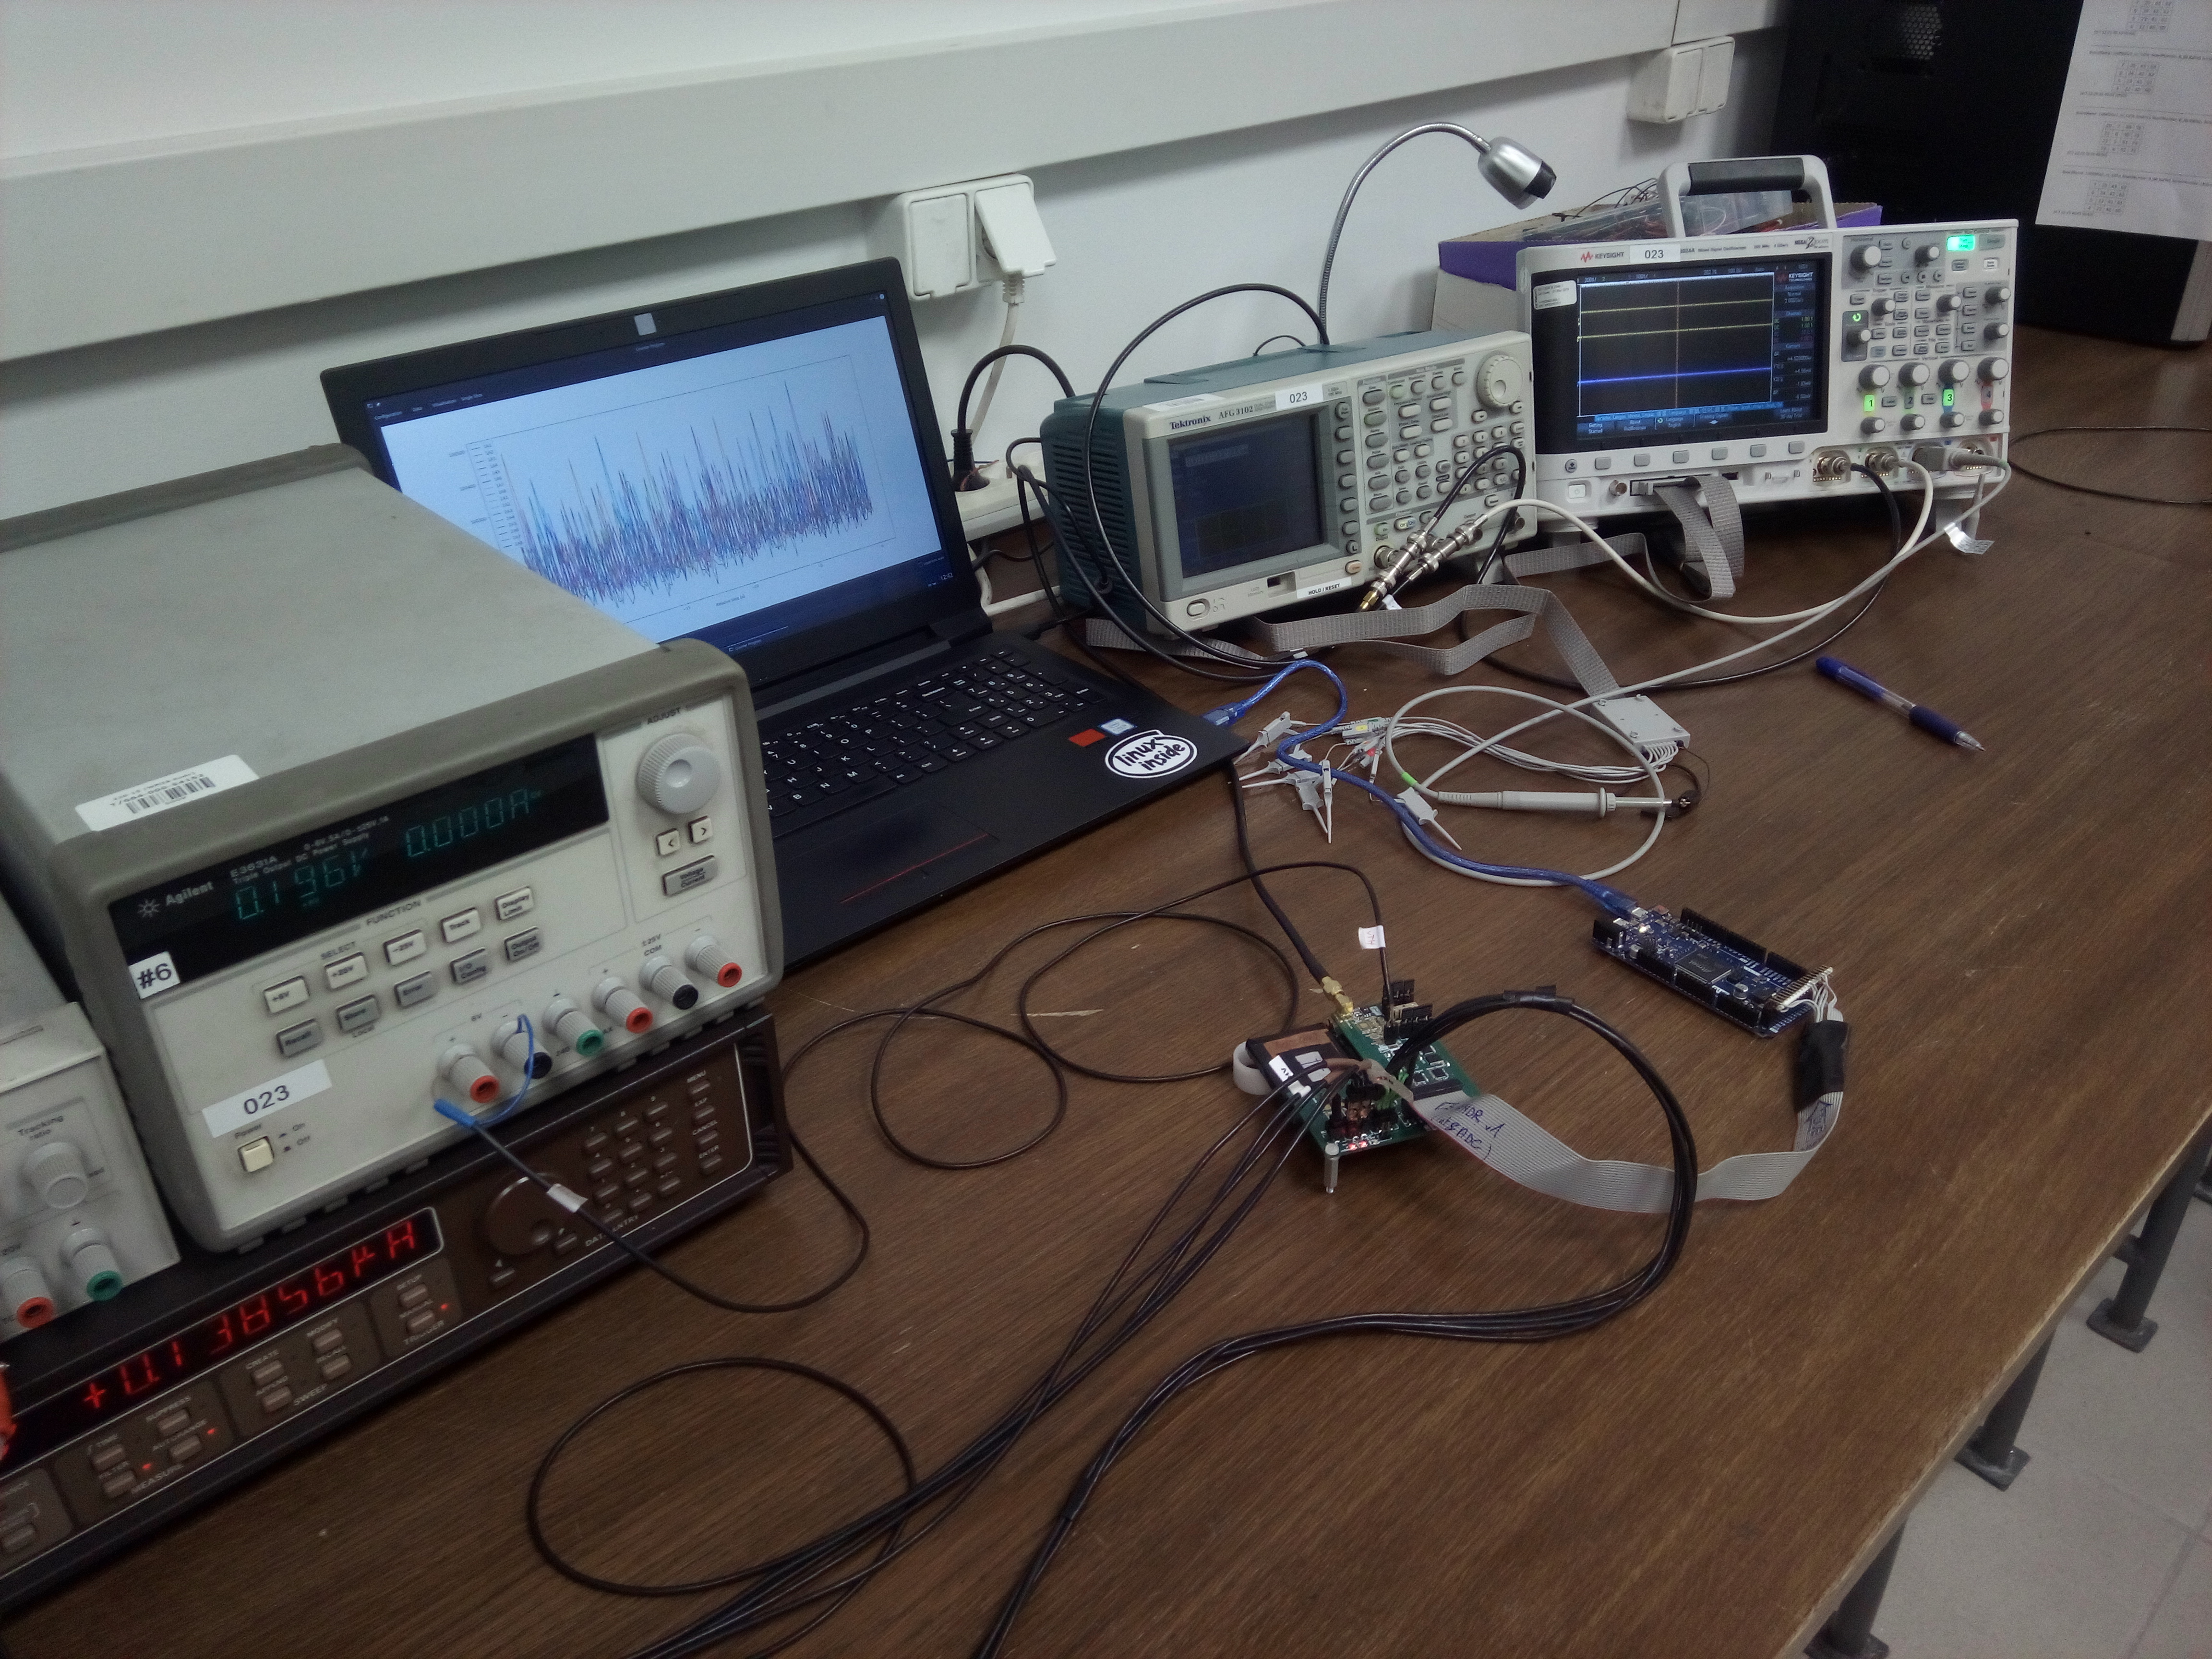
\includegraphics[width=0.5\textwidth]{setup.jpg}
            \caption{Zdjęcie funkcjonowania układu badawczego w trakcie pracy}
            \label{pic koniec} \par
            
        \end{multicols}
\end{figure}

Na przyszłość w projekcie można dokonać dodatkowe zmiany:
\begin{itemize}
        \item Dokładniejsze dopasowanie współczynnika czasu martwego z wykorzystaniem większej ilości kanałów do wyliczenia wartości $D_f$.
        \item Upewnienie sie o równej długości wszystkich cykli odczytu kanałów. Dopasowanie ilości pustych funkcji NOP dla kanałów 1A8 i 2A8.
        \item Uzależnienie wartości współczynnika WAIT\_FOR programu układu kontrolującego od wartości czasu akwizycji, pozwoliłoby to na pewniejszą kontrolę układu dla wysokich czasów akwizycji. 
        \item Uwzględnienie wydajności liczników w celu minimalizacji wariancji między kanałami. 
        \item Dodanie kontroli analogowej części odczytu impulsów układu RXHDR\_V1.
        \item Testy układu dla różnych długości cyklu pustego. 
        \item Wersja układu liczników nie zawierająca cyklu pustego. 
\end{itemize}
